\section{Interpretability}
\label{sec:interpretability}

Since the models in Table~\ref{tab:results} are about equally accurate, we ask three questions that accuracy cannot answer: what drives the submitted model, why the graph adds no accuracy, and whether the explanations can be trusted. We explain LightGBM with TreeSHAP \cite{Lundberg:2020:TreeSHAP}, which is exact for trees. We explain the neural models with Integrated Gradients (IG) \cite{Sundararajan:2017:IG}, which handles their thousands of inputs per rental, using 32 steps from an average flat in an average block. With all blocks equal at that baseline, the graph has nothing to pass on. The market level is a multiplier outside these networks, so time gets no attribution in them.

\subsection{Explaining the Submitted Model}

TreeSHAP on 5,000 test rows attributes 46\% of the submitted model's contributions to time, 31\% to flat attributes, 12\% to block premiums, 6\% to distance features and 5\% to the town. Time is large because SHAP compares each row with the average over all training months, and early months rented far lower. Excluding time, the shares are 57\%, 22\%, 12\% and 10\%. The time contribution also shows the frozen level directly: it rises from about $-\$660$ in January 2021 to about $+\$436$ in March 2025, then stays between \$433 and \$437 in the test months.

\subsection{Why the Graph Adds No Accuracy}

Here we explain the models of Table~\ref{tab:results} themselves: the GNN and the MLP with block premiums on the average level, retrained on the same epochs (each within 0.03 of its recorded RMSE), on 400 random holdout rentals. As a reference we use TreeSHAP on LightGBM with premiums on the same level. LightGBM has a different block table from the networks (Section~\ref{sec:gnn}), so we compare broad feature families.

Fig.~\ref{fig:importance} shows that the models broadly agree (Spearman 0.86 over seven families). Floor area and flat type lead, followed by block premiums (\$93 for the GNN, \$104 for LightGBM). LightGBM leans more on flat type (\$187 against \$127) and less on floor area (\$85 against \$144), and these two features overlap.

\begin{figure}[htbp]
\centerline{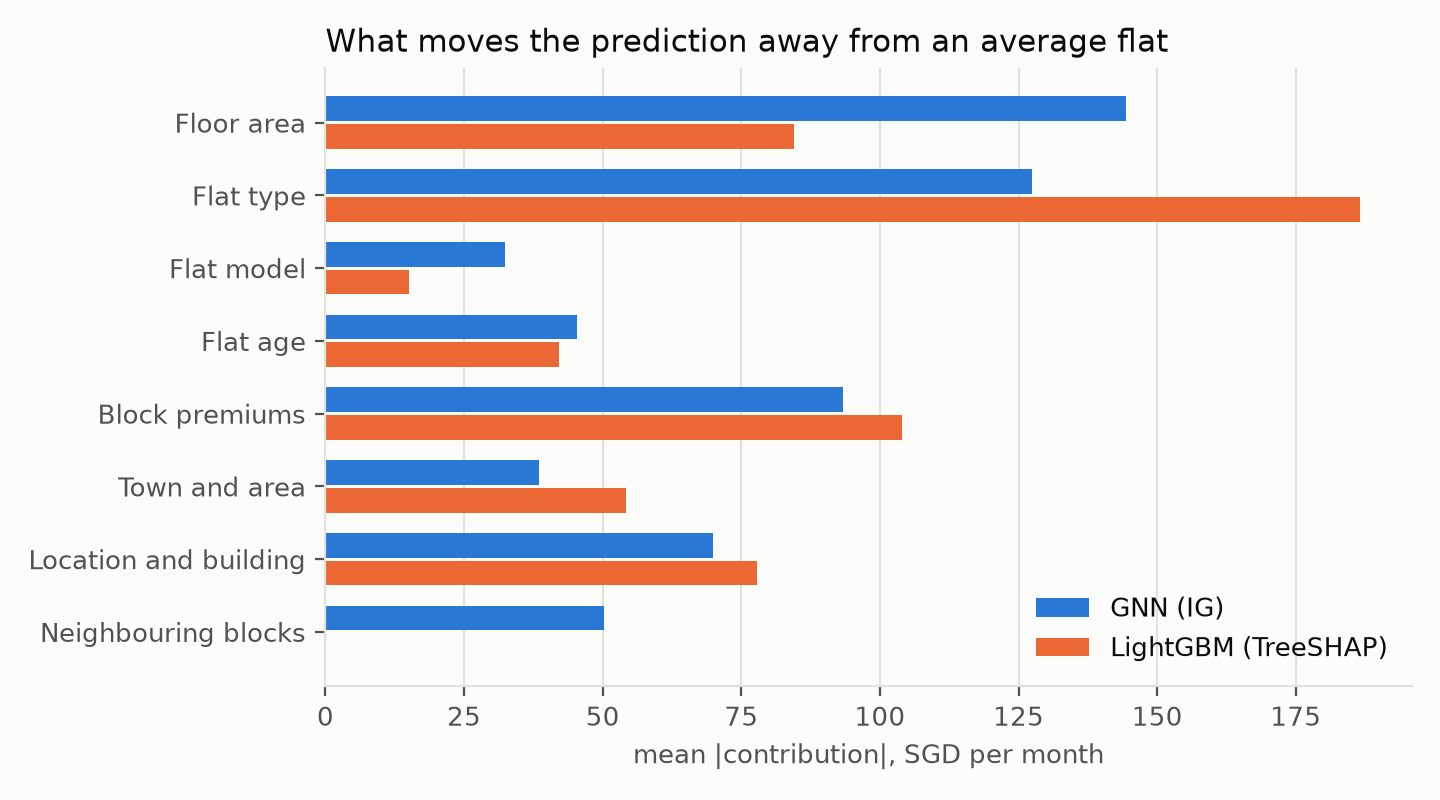
\includegraphics[width=\columnwidth]{figures/importance_table2.png}}
\caption{Mean absolute contribution by feature family for the models of Table~\ref{tab:results}: the GNN with premiums (IG) and LightGBM with premiums (TreeSHAP). LightGBM has no neighbours, so that bar has no counterpart.}
\label{fig:importance}
\end{figure}

Among these models, only the GNN can split credit among neighbouring blocks. Neighbours carry only location and amenity features through message passing. Premiums join at the head, so a neighbour's attribution never reflects its rents. Neighbours carry 17\% to 20\% of the absolute attribution over all inputs, or 8\% to 9\% when each family is first netted per rental, so the size of this share depends on how it is measured.

The GNN uses its neighbours but does not need them. Its location effect from its own block and neighbours (\$222) matches the MLP's from its own block alone (\$217), and the GNN's own block alone gives \$176. So neighbours repeat a signal that the block already has, which explains why the graph adds no accuracy. Their attributions show how credit is shared, and not that a neighbour is needed. Influence also stops at direct neighbours: \$5.4 on average for a direct neighbour and \$0.1 for one two hops away.

Fig.~\ref{fig:history} breaks this down by history. Neighbours' share is largest where it should be: with no earlier rentals of that block and flat type, neighbours (\$68) exceed the premium values (\$29), and the row count, which signals the missing history, carries \$68. But the block's own features remain largest (\$165), and the MLP, with no neighbours, simply puts more weight on them (\$263). With 3 to 5 rentals the premiums lead (\$118, against \$53 for neighbours).

\begin{figure}[htbp]
\centerline{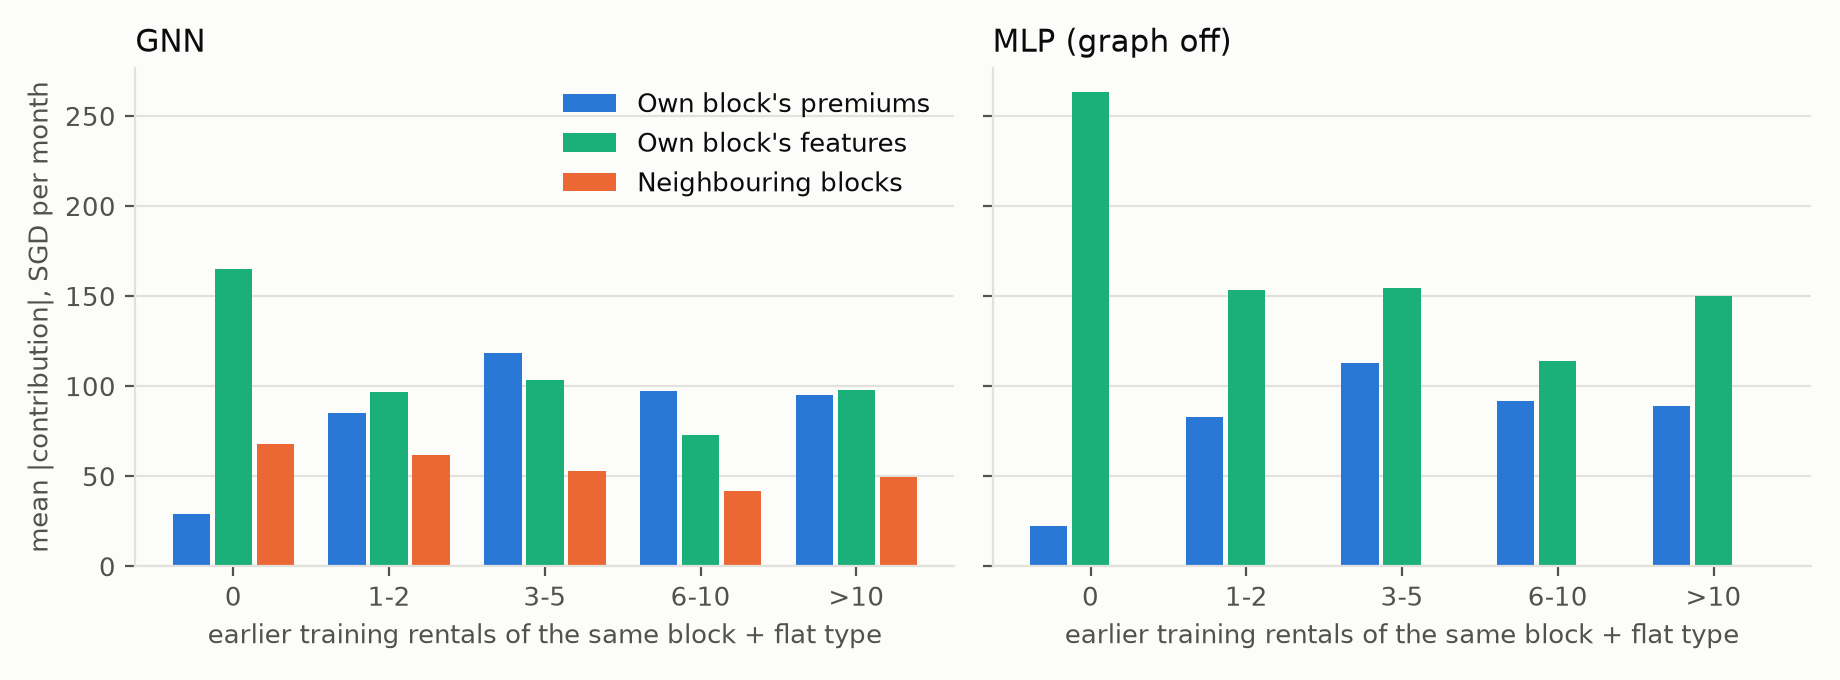
\includegraphics[width=\columnwidth]{figures/history_table2.png}}
\caption{Mean absolute contribution of a block's premiums (excluding the row count), its own features and its neighbours, by the number of training rentals of the same block and flat type, for 120 holdout rentals in each group.}
\label{fig:history}
\end{figure}

As a side test, we also explained a sibling model with the neighbours' premium channel of Section~\ref{sec:gnn}, on the damped trend level (482.1). With no history, neighbours' premiums moved a prediction by \$63, about as much as the block's own premium (\$68). The MLP with the same channel shows the same pattern (\$73 and \$66), so this comes from the premium input and not from message passing. This model only had the exactness checks below.

\subsection{Checking the Explanations}

We set no pass criteria in advance, so we report measured values, on the GNN of Table~\ref{tab:results} unless stated.

\emph{Mechanics.} The subgraph used for each rental matches the full graph to $2\times10^{-7}$. The median gap between a prediction's change and its attributions is under \$1, with a maximum of \$15. The MLP gets exactly \$0 on neighbours, which shows that the attributions are wired correctly.

\emph{Do attributions reflect the model?} Resetting the five most-attributed inputs moves a prediction by \$302 on average, against \$17 for five random inputs from the rental's own record and block. Family rankings agree across seeds (Spearman 0.87 to 0.89) and fall to 0.33 against an untrained network.

\emph{Do they rank individual neighbours?} This check is weaker. Across seeds, the ranking of a rental's direct neighbours agrees at 0.68 to 0.72, against 0.02 for an untrained network, so it is not noise. But resetting the top-ranked neighbour moves a prediction by only \$8.2, against \$5.9 for a random direct neighbour. We therefore trust the neighbours' total more than the ranking of any single neighbour, which in any case has little effect.

\emph{Does IG find a true effect?} The data has no ground truth for neighbours, so we planted one, on the GNN without premiums, since a block's premium would be expected to absorb a planted neighbour effect (Fig.~\ref{fig:planted}). This tests the method, not the model of Table~\ref{tab:results}, and only for a random effect unrelated to location, which is the easy case. On one seed, IG ranked neighbours well (0.93 against the truth, per neighbour), but reported about half of the effect's size. A control with nothing planted received \$3.8, and a pure noise input \$9. So IG finds direction and ranking in this setting, its dollar amounts for neighbours understate the effect, and differences under about \$9 should not be read as signal.

\begin{figure}[htbp]
\centerline{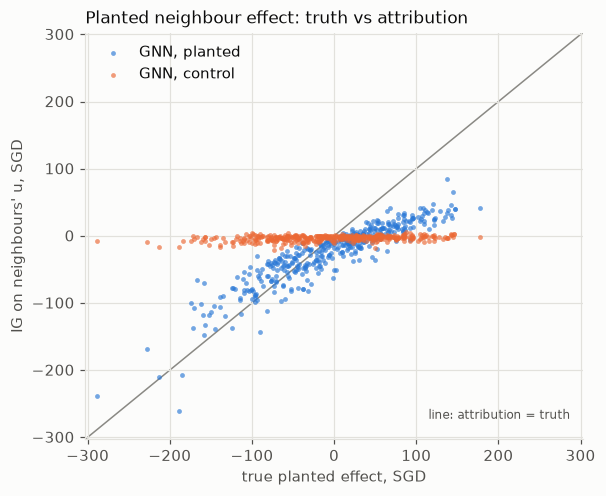
\includegraphics[width=0.85\columnwidth]{figures/planted_recovery.png}}
\caption{IG attribution on a planted neighbour value against the true planted effect, for a GNN without premiums trained on the planted target, and a control with nothing planted.}
\label{fig:planted}
\end{figure}
